\documentclass[a4paper,12pt]{article}
\usepackage[utf8]{inputenc}
\usepackage[MeX]{polski}
\usepackage{graphicx}
\hyphenation{oaza}
\hyphenation{oaza}
%opening
\title{Parafia św. Jerzego w Mszanie}
\author{Kamil Schilling}
\begin{document}

\maketitle

\begin{abstract}\noindent Parafia pw. św. Jerzego w Mszanie – rzymskokatolicka parafia w dekanacie jastrzębskim w archidiecezji katowickiej.
\end{abstract}

\begin{figure}[h]
\centering
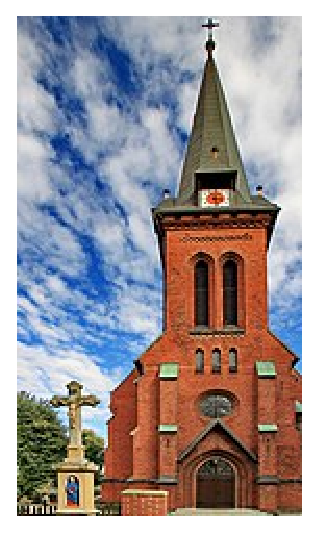
\includegraphics[width=0.3\hsize]{kos.eps}
\caption{Kościół}\label{kosciol}
\end{figure}

\section{Historia parafii}

Nie jest znana dokładna data powstania pierwszego kościoła, a~tym samym i parafii. Pierwsza wzmianka o miejscowości Mszana pochodzi z roku 1305. Parafia została po raz pierwszy wymieniona w~spisie świętopietrza sporządzonym przez archidiakona opolskiego Mikołaja Wolffa w 1447 pośród innych parafii archiprezbiteratu (dekanatu) w Żorach pod nazwą Mischna.
Wtedy to właśnie pobrano w Mszanie 5 groszy świętopietrza. Nie jest znany rok budowy pierwszego mszańskiego kościoła. Prawdopodobnie był pod wezwaniem św. Jerzego. Przetrwał do roku 1709, kiedy to zbudowano kolejny kościół, drewniany, któremu patronował również św. Jerzy. Kościół posiadał dwa dzwony, które zapewne pochodziły z poprzednich kościołów, jeden z roku 1520, drugi z roku 1557. Od XVI w. parafia należała do dekanatu wodzisławskiego. Pod koniec XIX wieku kościół został rozebrany, a~zamiast niego, w~1898 r. wybudowano z cegły nowy\footnote{Patrz Rysunek \ref{kosciol}}, który stoi do dnia dzisiejszego. Budowniczym kościoła był ks. Wilhelm Tusker, ówczesny proboszcz w Mszanie, którego grób znajduje się na cmentarzu parafialnym.

W~parafii działa Oaza Rodzin, III Zakon św. Franciszka, Zespół Charytatywny, Żywy Różaniec, Dzieci Maryi, Oaza młodzieżowa i liczna grupa ministrantów. W kształtowaniu życia wspólnoty parafialnej aktywną rolę odgrywa Parafialna Rada Duszpasterska. W~parafii ukazuje się pismo parafialne pt.,,Wiesiadni''. W~kościele, oprócz codziennych Mszy św., odprawiane jest w~każdą środę nabożeństwo do Matki Boskiej Nieustającej Pomocy, w~każdy czwartek odbywa się adoracja Najświętszego Sakramentu, a~w~każdą sobotę odmawiany jest Różaniec św. W~czasie wielkiego postu w roku 2005 parafia przeżywała Misje Święte prowadzone przez księży ze Zgromadzenia Misjonarzy Świętej Rodziny. Jesienią 2006 roku odbyła się kolejna wizytacja biskupia przeprowadzona przez Metropolitę Katowickiego – księdza arcybiskupa Damiana Zimonia.W~latach 2003-2004 w~miejscu starego probostwa wybudowano kaplicę przedpogrzebową, a~w~2008 roku dokonano remontu salek katechetycznych.


\begin{table}[h]
\centering \caption{Proboszczowie}
\begin{tabular}{lr}
\hline
ks. Rafał Greiff &(1971 – 1992)\\
ks. Alojzy Wyrwalec &(1992 – 2001)\\
ks. dr Jacek Wojciech& (2001 – 2009)\\
ks. Krystian Gawleński& (2009 – nadal)\\
\end{tabular}
\end{table}




\end{document}